\documentclass[11pt]{article}
\usepackage{amsmath}
\usepackage{amssymb}
\usepackage{color}
\usepackage{xcolor}
\usepackage{tikz}
\usepackage{pgfplots}
\pgfplotsset{width=10cm,compat=1.9}

\begin{document}

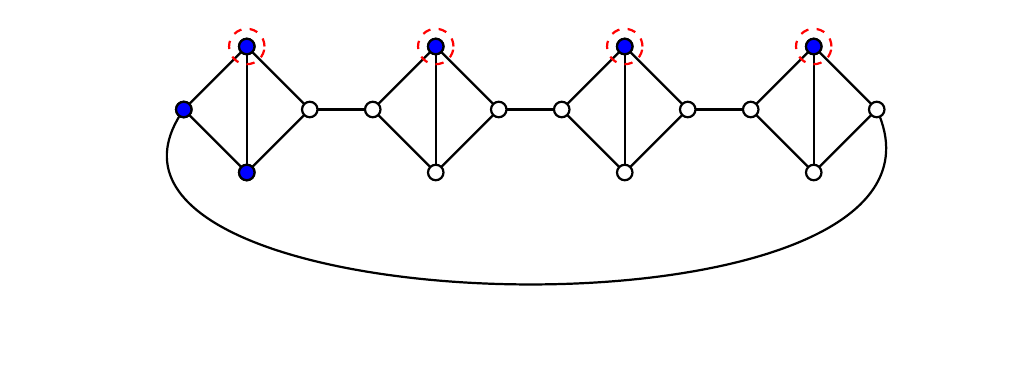
\begin{tikzpicture}[scale=.8,style=thick,x=1cm,y=1cm]
\def\vr{3.5pt}

% Define vertices for the diamond-necklace
\path (-.5, 0.0) coordinate (d11);
\path (0.5, 1.0) coordinate (d12);
\path (1.5, 0.0) coordinate (d13);
\path (0.5, -1.0) coordinate (d14);

\path (2.5, 0.0) coordinate (d21);
\path (3.5, 1.0) coordinate (d22);
\path (4.5, 0.0) coordinate (d23);
\path (3.5, -1.0) coordinate (d24);

\path (5.5, 0.0) coordinate (d31);
\path (6.5, 1.0) coordinate (d32);
\path (7.5, 0.0) coordinate (d33);
\path (6.5, -1.0) coordinate (d34);

\path (8.5, 0.0) coordinate (d41);
\path (9.5, 1.0) coordinate (d42);
\path (10.5,0.0) coordinate (d43);
\path (9.5, -1.0) coordinate (d44);

% % Draw the edges
\draw (d11) -- (d12);
\draw (d12) -- (d13);
\draw (d11) -- (d14);
\draw (d14) -- (d13);
\draw (d12) -- (d14);

\draw (d13) -- (d21);

\draw (d21) -- (d22);
\draw (d22) -- (d23);
\draw (d21) -- (d24);
\draw (d24) -- (d23);
\draw (d22) -- (d24);

\draw (d23) -- (d31);

\draw (d31) -- (d32);
\draw (d32) -- (d33);
\draw (d31) -- (d34);
\draw (d34) -- (d33);
\draw (d32) -- (d34);

\draw (d33) -- (d41);

\draw (d41) -- (d42);
\draw (d42) -- (d43);
\draw (d41) -- (d44);
\draw (d44) -- (d43);
\draw (d42) -- (d44);

% The curved edge
\draw (d11) to[out=-125,in=-65] (d43);

% Draw the vertices
\foreach \i in {1,2,3,4} {
    \draw (d\i1) [fill=white] circle (\vr);
    \draw (d\i2) [fill=white] circle (\vr);
    \draw (d\i3) [fill=white] circle (\vr);
    \draw (d\i4) [fill=white] circle (\vr);
}

\draw (d12) [fill=blue] circle (\vr);
\draw[dashed, red] (d12) circle (8pt);

\draw (d22) [fill=blue] circle (\vr);
\draw[dashed, red] (d22) circle (8pt);

\draw (d32) [fill=blue] circle (\vr);
\draw[dashed, red] (d32) circle (8pt);

\draw (d42) [fill=blue] circle (\vr);
\draw[dashed, red] (d42) circle (8pt);

\draw (d11) [fill=blue] circle (\vr);
\draw (d14) [fill=blue] circle (\vr);



\end{tikzpicture}

\end{document}